%Redigé par Théo Falgarone, Alexis Hubert, Tristan Maunier, Christian Té 
% * <chris33127@gmail.com> 2017-03-08T08:36:14.101Z:
%
% ^.

\documentclass[a4paper, 12pt]{report}
%
\usepackage[english,french]{babel} %Import french package for every keyword like Table of contents -> Table des matieres
\usepackage{float}
\usepackage[utf8]{inputenc}
\usepackage[Ot1,T1]{fontenc}
\usepackage[top=2.5cm, bottom=3cm, left=2.5cm, right=2.5cm]{geometry}
\usepackage{graphicx}


\setcounter{tocdepth}{3} %Limits depth in the table of content of sections showed
\setcounter{secnumdepth}{4} %Limits numerotation, in order to avoid Section 1.1.1.1.1...

\usepackage{listings} %Package that allow us to put code in the report

\begin{document}
	\begin{titlepage}
    	\begin{center}
		\vfill
		\Huge{OSS 117 : Eye Origin\\
        Cahier des charges}
		\vfill
		\end{center}
		\begin{center}
	        \centering
\includegraphics[height=3cm]{univ.jpg}\hfill \\
	    
		\LARGE{Université de Bordeaux}\\
		 Théo Falgarone, Alexis Hubert, Tristan Maunier, Christian Té \\
        Date de remise : 28/02/17

		\vfill
		\vfill
         \end{center}
                 \begin{minipage}{0.4\textwidth}
\begin{center} \large
\emph{Clients:} \\
Adrien \textsc{Boussicault} % Supervisor's Name
\par Pierre \textsc{Lacroix} % Supervisor's Name
\end{center}
\end{minipage}\\[2cm]
	\end{titlepage}
	
    %Create the table of contents
    \tableofcontents
    
    %We have to reset the counter because Introduction is always the page number 1
    \setcounter{page}{0} 
    	
	\chapter*{Introduction} %The star protects the chapter to be counted
		\addcontentsline{toc}{chapter}{Introduction} 
L'objectif de ce projet est de concevoir un paquet regroupant un logiciel de suivi du mouvement des yeux et un gestionnaire de fenêtre qui permettraient de faciliter l'utilisation d'un ordinateur aux personnes à mobilité réduite qui sont dans l'incapacité physique d'utiliser une souris et un clavier. Pour cela le logiciel doit, à l'instar d'une souris classique, permettre à l'utilisateur de pouvoir diriger le pointeur sur l'écran via une reconnaissance du mouvement de l'iris. L'utilisateur doit également pouvoir utiliser ce pointeur pour utiliser un clavier virtuel générer par le gestionnaire de fenêtre. \\

Notre projet reprends une grande partie du travail déjà effectuée l'an passé par nos collègues de Master 2, le projet OSS 117\cite{c7}.


                %The way to include pictures
                %{\centering\includegraphics[height=1.25cm]{distance.png}\par}
    \chapter{Les besoins}
		\section{Les besoins fonctionnels}
        \subsection{Comparaison d'algorithmes permettant la détection de l'iris}
\begin{enumerate}
\item \textbf{Créer une librairie d'images de visages recueillies selon un protocol prédéfini. La librairie d'images devra être utilisable pour les algorithmes qui pourraient être testés}
\item \textbf{Etablir un protocole de collecte des images pouvant être reproductible. Ce protocole devra respecter les besoins suivants :}
\begin{enumerate}
\item Définir différentes positions pour la caméra
\item Définir différents points de repères sur l'écran.
\item Définir différents angles (verticaux et horizontaux) pour la caméra.
\item Construire un dispositif permettant de placer la caméra aux différentes positions et angles prédéfinis.
\item Définir la position de l'utilisateur vis à vis de la caméra et de l'écran.
\end{enumerate}
\item \textbf{Concevoir un programme qui permettra à l'utilisateur, via un événement click souris, de renvoyer les coordonnées des centres des iris de chaque image de la librairie dans un fichier.}
\item \textbf{Concevoir un programme qui intégrera un algorithme de détection de l'iris et qui retournera les coordonnées des centres des iris dans un fichier. Le programme devra être facilement modifiable pour pouvoir y integrer différents algorithmes}
\item \textbf{Interpréter les deux jeux de données afin de déterminer si l’algorithme fonctionne et dans quelles conditions (positions de caméra, angles). Cette interpretation sera effectuée par le biai de tests statistiques propres aux traitements d'images. Et les critères d'évaluation devront pouvoir être modifiés facilement.}
\item \textbf{Déterminer une corrélation entre les différentes positions de la caméra (définies dans le protocole) et la bonne détection du centre de l’iris dans les images}
\end{enumerate}
        \subsection{Détection de l'iris}
\begin{enumerate}
\item \textbf{Capturer un flux d'images via une caméra }
\item \textbf{Reconnaître l'iris :}
\begin{enumerate}
\item Reconnaître le visage de l'utilisateur afin de repérer ses yeux à partir du flux d'images récupéré 
\item Reconnaître les yeux à partir de la zone de détection du visage
\item Choisir un oeil afin de réduire la quantité de données à gérer
\item Reconnaître l'iris dans la zone de détection de l'oeil
\end{enumerate}
\end{enumerate}
		\subsection{Interpretation des mouvements de l'iris}
\begin{enumerate}
\item \textbf{Déterminer la position de l'iris dans le flux d'images, sous forme de coordonnées.}
\item \textbf{Interpréter les coordonées de l'iris pour déplacer le curseur}
\item \textbf{Lancer une fenêtre qui permettra de calibrer le déplacement du curseur en fonction de la taille de l'écran.}
\item \textbf{Calibrer la position de l'écran par rapport à l'utilisateur grâce à des repères spatiaux}
\end{enumerate}
		\subsection{Affichage}
\begin{enumerate}
\item \textbf{Ajouter un curseur de souris dans un gestionnaire de fenêtre }
\item \textbf{Afficher un clavier virtuel dans la partie basse de l'écran.}
\item \textbf{Permettre de réaliser des clicks souris (click droit, click gauche, double click et copier-coller) grâce à des touches spécifiques situées sur le clavier virtuel apparaissant à l'écran.}

\end{enumerate}
        \section{Les besoins non fonctionnels}
\begin{enumerate}
\item \textbf{Integrer OSS dans les gestionnaires de fenêtres usuels}
\begin{itemize}
\item Gnome
\item Kde
\item Unity
\item Xfce
\end{itemize}
\item \textbf{Empêcher le chevauchement des fenêtres sur le clavier virtuel}
\end{enumerate}
\chapter{Projet OSS 117}
    Le projet OSS 117 a été conçu pour fonctionner via une webcam, comme celles intégrées dans la plupart des ordinateurs portables. Le logiciel est écrit en C++\cite{c8} (langage de programmation orientée objet) et utilise une librairie graphique de traitement d'image OpenCV. En plus du eye-tracking, le projet OSS 117 inclut un gestionnaire de fenêtre (DWM) affichant un clavier virtuel en bas de l'écran permettant à l'utilisateur de s'affranchir aussi de l'utilisation du clavier. Malheureusement, le logiciel ne permet pas de déplacer la souris via les mouvements de l'iris. Quand bien même une majorité du travail effectué pourra être reprise et constituera une base solide pour notre projet. Revenons sur le fonctionnement générale du logiciel et listons les points que nous pouvons conserver et ceux que nous devrons modifier ou ajouter.
    
    	\section{Architecture OSS 117}
        Premièrement le logiciel prévoit un calibrage, une série de points apparaissant à l'écran que l'utilisateur devra regarder successivement permet d'analyser le mouvement	 de l'iris à des positions pré-déterminées. Ces coordonnées de référence servent à déplacer le curseur en fonction du mouvement de l'iris. Ensuite il s'agira d'analyser puis d'interpréter le mouvement de l'iris via la caméra et le traduire en déplacement du curseur sur l'écran en se basant sur les données présentes dans le fichier de calibration. \\
        
\begin{figure}[H]
\centering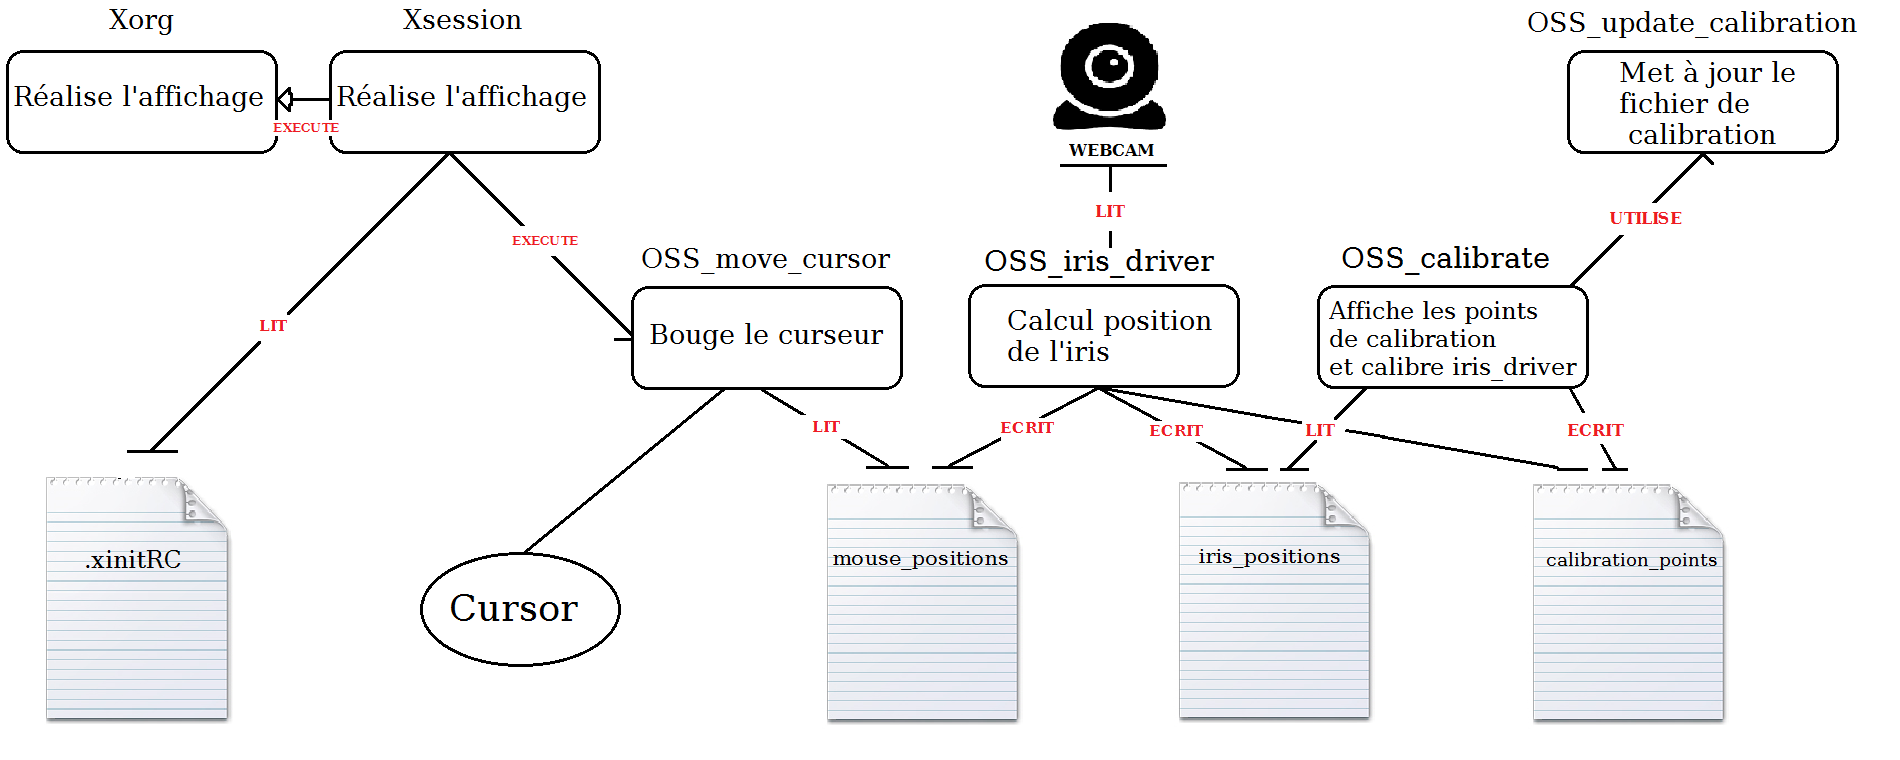
\includegraphics[height=6cm]{algoOSS.png}
\caption{UML Programme OSS 117}
\end{figure}
        
	\chapter{Etat de l'art}
    \section{Eye tracking}
 
\begin{itemize}
\item Tobii\cite{c1} eyeX : c'est une barre à placer en dessous de l'écran, dotée de deux caméras et de 3 led InfraRouge permettant le suivi des yeux et de déplacer la souris à l'écran. Il est utilisé pour la navigation sur l'ordinateur et les jeux vidéos. Le logiciel est propriétaire.
\end{itemize}
\begin{figure}[!ht]
\centering
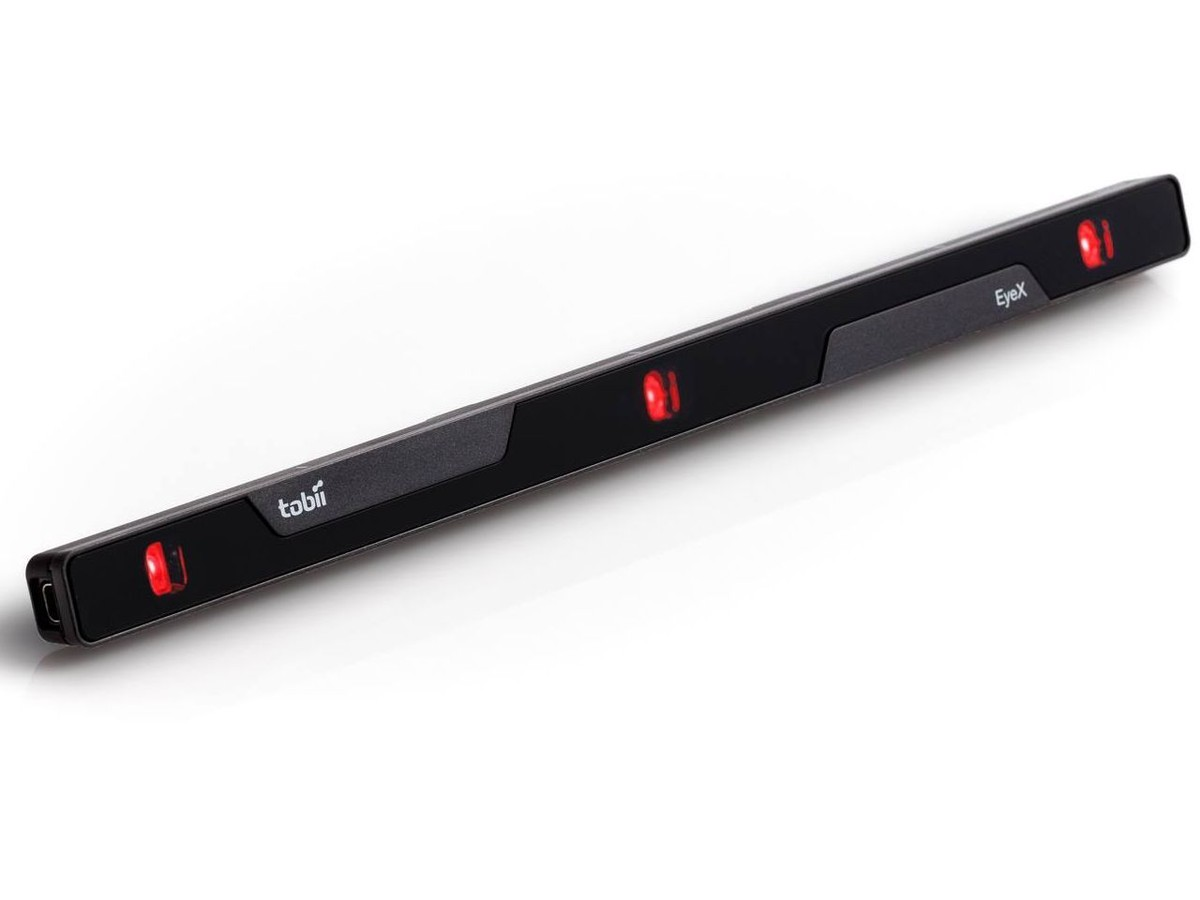
\includegraphics[height=4cm]{tobii.jpg}
\caption{Tobii eyeX \textasciitilde 200\$}
\end{figure}
\begin{itemize}
\item Smart Eye\cite{c2} Pro 5.0 : nécessite 2 à 8 caméras dotées de led InfraRouge. Conçu dans un but de recherche, il permet un suivi des yeux précis afin d'identifier les zones d'intérets de l'utilisateur et d'autres informations concernant son regard.
\end{itemize}
\begin{figure}[!ht]
\centering
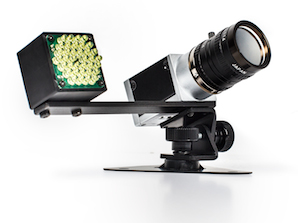
\includegraphics[height=4cm]{Smarteye.jpg}
\caption{Smart Eye}
\end{figure}
\newpage

\underline{Imotions\cite{c3}}\\
\par Logiciel de détection des yeux qui permet de faire une cartographie des régions d'intéret de l'utilisateur, de quantifier l'attention visuel (par le temps passé) ainsi que de mesurer la dilatation des pupilles. Il a pour but d'analyser des zones d'intérets de sites internets, ou dans les rayons d'un supermarché. Il a donc un but commercial.\\

\underline{EyeLike\cite{c17}}\\
\par EyeLike est un logciel permettant la detection la position de l'iris ansi que son mouvement au cours du temps. Ce logiciel ne nécessite qu'une simple webcam pour fonctionner et son code est open source.\\

\underline{EyeWriter\cite{c4}}\\
\par C'est un projet dont le but est de permettre à des personnes handicapées moteur de pouvoir dessiner à l'aide des yeux. Le dispositif de suivi de l'oeil est composé d'une caméra et de LEDInfraRouge qui peuvent être montés soit sur une barre à placer sous l'écran, soit directement sur des lunettes. Le logiciel est divisé en deux parties, le Eye-Tracking et le Eye-Drawing. Le Eye-tracking est basé pour la calibration sur la Gnu Scientific Library\cite{c6}. Le dispositif est relativement facile à créer et peu cher. Les instructions de construction sont accessibles.  Les logiciels quant à eux sont open source en General Public Licence. Tout le projet est libre de droits.
\begin{figure}[!ht]
\centering
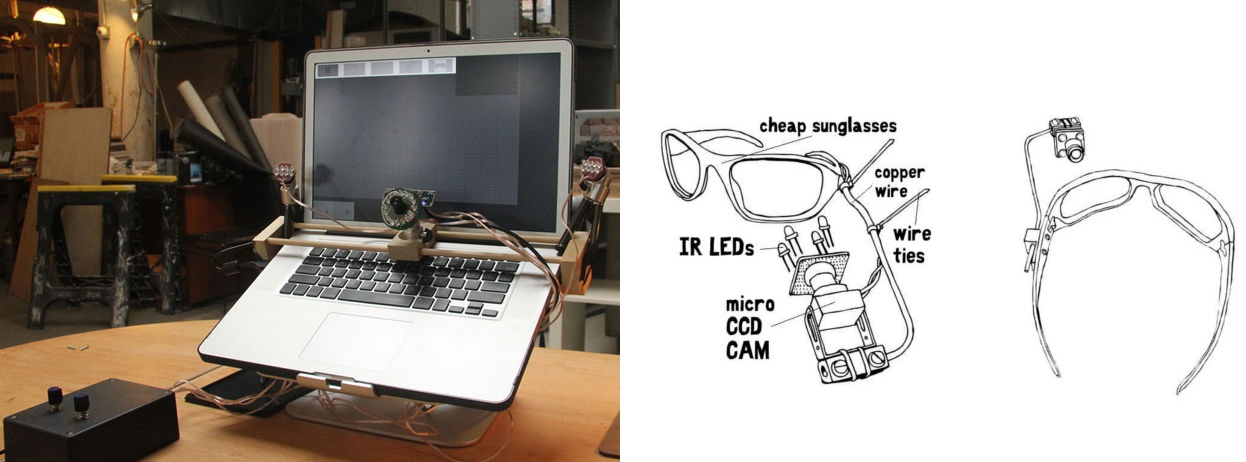
\includegraphics[height=5cm]{camw.jpg}
\caption{A gauche: EyeWriter 2.0, A droite: Eyewriter 1.0}
\end{figure}

\underline{INSA-Strasbourg\cite{c5}}\\
\par La publication date du 23 janvier 2017.
L'équipe de génie électrique de l'INSA de Strasbourg a mit au point un programme Matlab qui effectue le déplacement du curseur grâce au suivi des yeux. Le dispositif utilisé est uniquement une webcam. Le programme effectue dans un premier temps la capture d'images, la transformation de celles-ci en niveau de gris, puis la détection du visage. Ensuite il y a la détection des yeux dont ils retirent la position permettant ensuite de transcrire la direction au curseur. Leur programme travaillant dans Matlab, il ne permet donc pas d'agir en dehors de son environnement. Toute interaction avec l'ensemble de l'espace de travail de l'ordinateur est donc impossible. Tous droits réservés INSA 2017.

\newpage
\section{Face tracking}
\begin{itemize}
\item \textbf{Enable Viacam\cite{c14} :}
\begin{figure}[!ht]
\centering

\includegraphics[height=2.5cm]{index.jpeg}
\end{figure}
\\Enable Viacam (eViacam) est un logiciel qui permet de contrôler la souris simplement en bougeant la tête.Il fonctionne sur des PC standard équipés d'une webcam. Aucun autre matériel supplémentaire n'est nécessaire. Il est gratuit et opensource.
\end{itemize}

    \chapter{Charges}
Nous avons décidé de réaliser les besoins fonctionnels cités en 1.1.1 Comparaison des algorithmes de détection de l'iris, à la page 2:
\begin{enumerate}
\item Mise au point du protocole d'acquisition des images pour construire la librairie.
\begin{itemize}
\item Définir les différentes positions de la caméra autour de l'écran, les différents points de repères sur l'écran et les angles d'inclinaison de la caméra.
\item Construire un dispositif permettant de positionner la caméra sur les différentes positions définies. Ce dispositif permettra également de modifier l'angle d'inclinaison de la caméra.
\item Mise aux points de consignes d'utilisation pour l'utilisateur.
\end{itemize}
\item Construction de la collection d'images
\item Conception d'un plugin imageJ qui permet, grâce à des clicks souris, de récupérer les coordonnées des centres des deux iris de chaque photo de la collection et de les écrire dans un fichier.
\item Conception d'un programme integrant l'algorithme testé et renvoyant les coordonnées des centres des deux iris de chaque photo de la librairie dans un fichier.
Algorithmes testés :
\begin{itemize}
\item Algorithme du programme EyeLike : adapté d'après l'algorithme de détection de l'iris de Tristan Hume.
\item
\end{itemize}
\item Conception d'un programme permettant de récupérer les deux jeux de coordonnées et de les comparer afin de déterminer si elle sont identiques ou non, une marge d'erreur sera prise en compte.
\end{enumerate}
\begin{figure}[!ht]
\centering
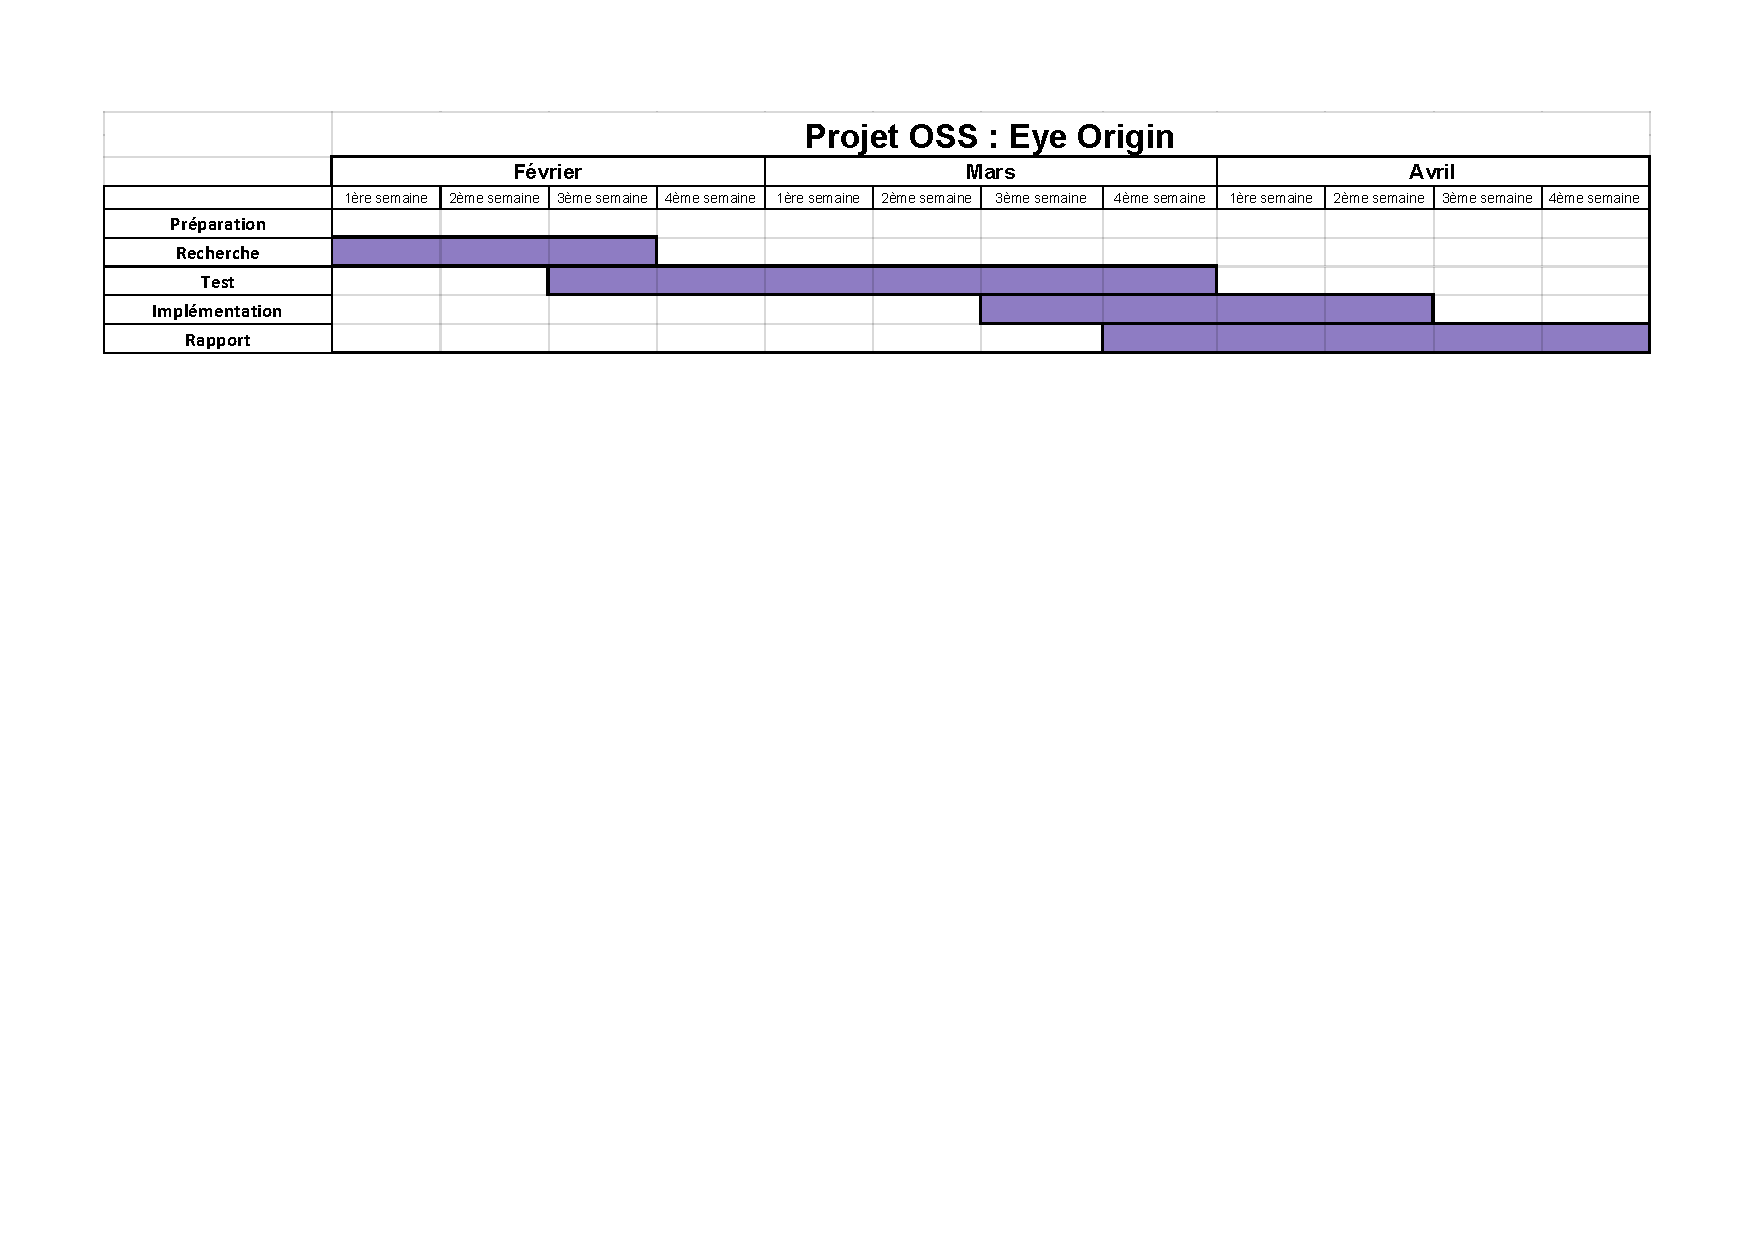
\includegraphics[height=12cm]{Diagrame.pdf}
\vfill
\caption{Diagramme de Gantt}
\end{figure}

        \centering
            \begin{thebibliography}{}
\addcontentsline{toc}{chapter}{References}
\bibitem{c7} Auteurs: Julien Estebeteguy, Lisa Perus, Alexandre Petit, Thomas Riquelme
\bibitem{c8} C++,Bjarne Stroustrup,1983
\bibitem{c1} tobii, http://www.tobii.com/tech/products/
\bibitem{c2} Smart Eye, http://smarteye.se/
\bibitem{c3} imotions, https://imotions.com/
\bibitem{c17} Tristan Hume. eyelike : A webcam based pupil tracking implementation. https:
//github.com/trishume/eyeLike.
\bibitem{c4} EyeWriter, http://www.eyewriter.org/
\bibitem{c5} GPL, https://www.gnu.org/licenses/licenses.fr.html
\bibitem{c6} INSA-Strasbourg, http://genie-electrique.insa-strasbourg.fr/projet-ge-alternance-eye-tracking/, 21 janvier 2017
\bibitem{c14} Enable Viacam.http://eviacam.sourceforge.net/index\_fr.php

\bibitem{c11} Unity. https://doc.ubuntu-fr.org/unity.
\bibitem{c12} Suckless. Dwm. http://dwm.suckless.org/.
\bibitem{c13} Gnome. Gnome. https://www.gnome.org/.
\bibitem{c16} Xfce, Olivier Fourdan , 1996
\bibitem{c15} Kde, Projet KDE, 1996





\end{thebibliography}{}
\end{document}%Redigé par  Théo Falgarone, Alexis Hubert, Tristan Maunier, Christian Te 

\documentclass[a4paper, 12pt]{report}

\end{document}